% This example is meant to be compiled with lualatex or xelatex
% The theme itself also supports pdflatex
\PassOptionsToPackage{unicode}{hyperref}
\documentclass[aspectratio=1610, professionalfonts, 9pt]{beamer}
\usefonttheme[onlymath]{serif}

% Load packages you need here
\usepackage{polyglossia}
\setmainlanguage{english}

\usepackage{csquotes}

\usepackage{amsmath}
\usepackage{amssymb}
\usepackage{mathtools}
\usepackage{unicode-math}
\usepackage{siunitx}

\usepackage{hyperref}
\usepackage{bookmark}

\usepackage{tikz}
\usepackage{feynman-tikz}

\usepackage{xparse}
\usepackage{braket}
\usepackage{ulem}
% \usepackage{units}

\usepackage{bookmark}
\usepackage{subfigure}
\usepackage{multicol}

\usepackage{animate}
\usepackage{graphicx}

\usepackage[style=verbose, backend=biber]{biblatex}
\usepackage{filecontents}% to embed the file `lit.bib` in your `.tex` file

% \usepackage{appendixnumberbeamer}


% load the theme after all packages
%\def\darktheme{1}
\ifdefined\darktheme
  \usetheme[
    % showtotalframes, % show total number of frames in the footline
  ]{tudo_dark}
\else
  \usetheme[
    % showtotalframes,
  ]{tudo}
\fi

% package settings
\unimathsetup{
  math-style=ISO,
  bold-style=ISO,
  sans-style=italic,
  nabla=upright,
  partial=upright,
  mathrm=sym,
}

\sisetup{
  separate-uncertainty=true,
  per-mode=reciprocal,
  output-decimal-marker={.},
  range-phrase = \text{--},
}
\DeclareSIUnit\crab{Crab}

% tikz settings
\usetikzlibrary{overlay-beamer-styles,calc,tikzmark,decorations.pathreplacing}
\tikzset{fontscale/.style = {font=\relsize{#1}}}

\setmathfont{XITS Math}[range={scr, bfscr}]
\setmathfont{XITS Math}[range={cal, bfcal}, StylisticSet=1]

\begin{filecontents*}{\jobname.bib}
@mastersthesis{hackfeld,
  author      = {Hackfeld, J.},
  title       = {Analyzing the Data Volume Reduction for the LST-1 Prototype of the Cherenkov Telescope Array},
  % institution = {Department of Physics and Astronomy, Ruhr University Bochum},
  year        = {2021},
  address     = {Bochum}
}
@online{perezdiaz,
  author       = {Pérez Diaz, G.},
  year         = {2016},
  url          = {https://www.cta-observatory.org/about/how-cta-works/},
  organization = {CTA/ IAC},
  urldate      = {2022-07-10}
}
\end{filecontents*}
% reference source
\addbibresource{\jobname.bib}


% This adds a circle with a picture of your choice in it.
% Usage:
% \roundpic[<optional arguments>]{<radius of the cirlce [cm]>}{<picture width [cm]>}{<path_to_picture>}{x pos}{y pos}
\newcommand{\roundpic}[6][]{%
  \node [circle, draw, color=tugreen, minimum width = #2,
    path picture = {
      \node [#1] at (path picture bounding box.center) {
        \includegraphics[width=#3]{#4}};
    }] at (#5,#6) {};}%

% Comment this out to represent vectors with an arrow on top.
% Uncomment this to represent vectors as bold symbols.
\renewcommand{\vec}[1]{\mathbf{#1}}


\newcommand{\yaml}[2]{%
  \texttt{\textcolor{#1}{\detokenize{#2}}}%
}

\title{Finding optimal hyperparameters for cleaning algorithms for the Cherenkov Telescope Array}
\subtitle{Bachelor thesis half-time talk}
\author[A.~Knierim]{Anno Knierim}
\date{July 15, 2022}
\institute[E5b]{E5b Astroparticle Physics \\  Department of Physics -- TU Dortmund}


\begin{document}

\maketitle

\begin{frame}{Table of contents}
  \tableofcontents
\end{frame}

\section{About this theme}
\begin{frame}{Notes}
  This theme is based on the excellent \texttt{TUDoBeamerTheme} provided by Maximilian Nöthe \texttt{https://github.com/maxnoe/TUDoBeamerTheme}.
  I merely added the dark theme option as well as some extras I found useful or "nice to have" when I created some talks with the original theme.
  \begin{itemize}
    \item To install this theme at least the files \texttt{beamerthemetudo.sty} and \texttt{beamerthemetudo\_dark.sty} as well as the folder logos have to be moved to a folder where \LaTeX{} can find packages.
      This can be
      \begin{itemize}
        \item \texttt{TEXMFHOME/tex/latex/tudobeamertheme} and \texttt{TEXMFHOME/tex/latex/tudobeamertheme\_dark}. You can get \texttt{TEXMFHOME} by running \texttt{kpsewhich --var-value TEXMFHOME}, usually this would be \texttt{\$HOME/texmf}.
        \item The same folder in which you compile your document.
        \item Any folder that is included in the variable \texttt{TEXINPUTS} (see \texttt{makefile}).
      \end{itemize}
  \end{itemize}

  One liner for installation:\\
  \texttt{\footnotesize\$ cd `kpsewhich --var-value TEXMFHOME` \&\& git clone https://github.com/aknierim/tudobeamertheme\_dark}

  \medskip
  General information on \LaTeX{} and Beamer:
  \begin{itemize}
    \item Extensive course on \LaTeX{} by PeP et Al. \\
      \url{http://toolbox.pep-dortmund.org/notes}
    \item Beamer \LaTeX{} class documetation:\\
      \url{http://www.ctan.org/pkg/beamer}
  \end{itemize}
\end{frame}


\section{Fonts}
\begin{frame}
  The font recommended in the corporate design of the TU Dortmund university
  is \enquote{Akkurat Office}.\\
  \bigskip
  If that font is not available, \enquote{Fira Sans} will be used as an alternative.\\
  \bigskip
  When using \texttt{xelatex} or \texttt{lualatex} the font \enquote{Latin Modern Math}
  will be used as a default but can be changed to \enquote{Fira Math} if you want a
  sans serif font.
\end{frame}

\section{Sample slides}
\subsection{Theory}
\begin{frame}{Some maths}
  Maths fonts can be set in \texttt{beamerthemetudo.sty} or \texttt{beamerthemetudo\_dark.sty}.
  Currently this is set to \enquote{Latin Modern Math}. Look for \texttt{\textbackslash setmathfont\{\}}
  to set a different math font.
  \begin{align*}
    \nabla \cdot \vec{B} &= 0 &
    \nabla \cdot \vec{E} &= \frac{ρ}{ε_0} \\
    \nabla \times \vec{E} &= -\partial_t \vec{B} &
    \nabla \times \vec{B} &= μ_0 \vec{j} + μ_0 ε_0 \partial_t \vec{E} &
  \end{align*}
\end{frame}

\subsection{Results}
\begin{frame}{Plot}
    This theme also comes with a \texttt{darkmode.mplstyle} that allows you to create
    plots fitting the dark or light theme (see \texttt{plots/darkmode.mplstyle}). The style will
    be applied automatically when running \texttt{make <all | light | dark>}.
  \begin{figure}
    \centering
    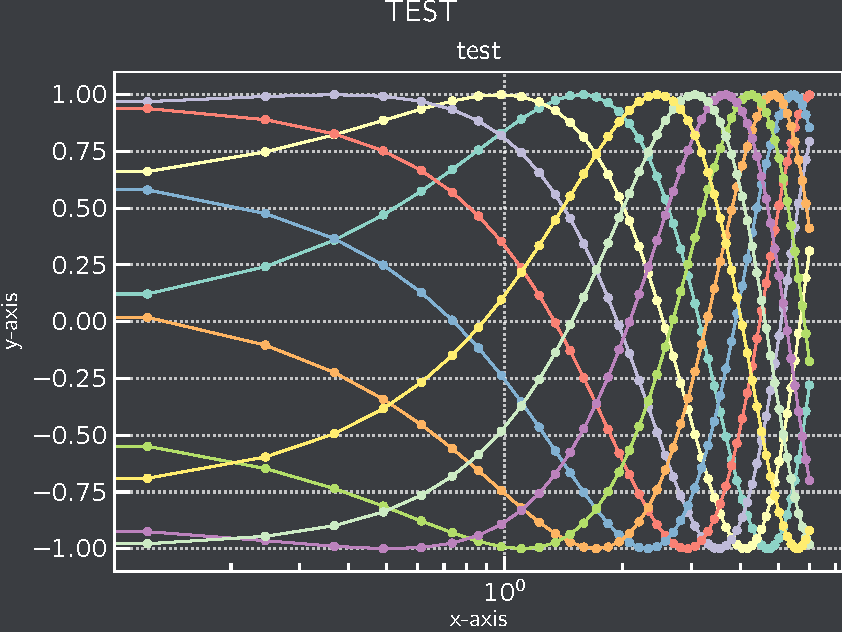
\includegraphics[height=0.75\textheight]{plots/plot.pdf}
  \end{figure}
\end{frame}


\end{document}
